\section{Partial Differential Equations (PDE)}\label{sec:pde}
A partial differential equation (PDE) is defined as a differential equation that relates the derivatives
of a function such that it depends on more than one independent variable.\cite{olver_2014_pde}
This project will look at two significant classes of PDEs, namely the heat equation and the Black-Scholes equation.

\subsection{Heat Equation}\label{sec:heat}
The heat equation describes how temperature diffuses through a medium over a period of time. 
Let $u(x, \tau)$ be the temperature of a medium 
at a specific point $x$ and time $\tau$.
We denote the derivatives of $u$ with respect to $\tau\geq 0$ 
and $x\in\R$ by $u_\tau$ and $u_x$, respectively.
The heat equation \cite{leveque_2007} states that 
\begin{equation}
u_{\tau} = \kappa u_{xx}, \label{eq:heat-equation}
\end{equation}
where $\kappa$ is the thermal diffusivity constant.
The initial and boundary conditions must be defined to obtain appropriate solutions to the heat equation. 

\subsubsection{Initial and Boundary conditions over a finite interval}
For the heat equation, the initial condition is specified by
\begin{equation}
u(x,0) = u_0(x),
\end{equation}
which describes the initial temperature across the length of the medium at time $t = 0$.

Assuming that the temperature distribution falls within a finite domain, the \textit{Dirichlet} boundary conditions are applied at the extreme ends of the domain \( (0 \leq x \leq L) \), that is,
\begin{subequations}
\begin{align}
u(0,t) ={}& \alpha(t),\\
u(L,t) ={}& \beta(t).
\end{align}
\end{subequations}
For the initial and boundary conditions to be 
well posed, they need to agree at $t=0$, $x=0$, 
and $x=L$
\begin{gather*} 
\alpha(0) = u_0(0), \\
\beta(0) = u_0(L).
\end{gather*} 


\subsection{Black-Scholes Equation}\label{sec:bse}
The Black-Scholes (BS) equation is the PDE
\begin{equation}
\frac{\partial V}{\partial t} + \frac{1}{2} \sigma^2 S^2 \frac{\partial^2 V}{\partial S^2} + r S \frac{\partial V}{\partial S} - r V = 0, \label{eq:black-scholes}
\end{equation}
where \( V(S,t) \) is the price of the call/put option at time $t$ given the price of the underlying asset, $S$, 
$t$ is the time elapsed since the creation of the option, 
$r$ is the risk-free interest rate, and
$\sigma$ is the volatility of the underlying.
Based on the type of option, the BS equation is accompanied by certain terminal and boundary conditions.

\subsubsection{European Call Option}
For European call options, we use the lower boundary condition (at $S=0$)
\begin{equation}
        V(0,t) = 0, 
\end{equation}
which means that the value of option for a zero-value underlying is zero.
An ``upper'' boundary condition is also imposed (at $S \rightarrow  \infty$).
% The upper condition enforces that for ``very expensive'' underlying assets, 
% the option should be priced at the same value as the underlying. 
% In other words, $V(S,t) \sim S$ as $S \to  \infty$.
Practically, this condition can be imposed at a sufficiently
large value $S_{\rm max}$. A typical choice \cite{kwok_2008_derivatives} is 
\begin{equation}
        V(S_{max},t) = S_{\rm max} - Ke^{-rT}.
\end{equation}
The term $Ke^{-rT}$ represents the present value of the strike price discounted by the the risk-free
rate $r$ over the time to expiry $T$. Lastly, we impose the terminal condition (at $t = T$),
which is 
\begin{equation}
 V(S_T,T) = \max(S-K,0)   
\end{equation}
for all $S$.
The option payoff $V(S,T)$ is specified at expiration $T$,
where $S$ represents the current price of the asset and $K$ denotes the strike price.

\subsubsection{European Put Option}
The case of European put options follows a different set of terminal and boundary conditions. Given the underlying asset
value at zero, the payoff becomes approximately $K$ when the option is exercised. Hence, we have
the lower boundary condition
\begin{equation}
    V(0,t) = Ke^{-rT}.
\end{equation}
On one hand, as the underlying asset $S$ becomes very large, the put option becomes inherently worthless which gives 
the upper boundary condition ($S \to \infty$)
\begin{equation}
    V(S,t) \to 0. 
\end{equation}
The terminal condition for the put option is set to
\begin{equation}
    V(S,T) = \max(K-S,0)
\end{equation}

\subsection{Equivalence between the heat equation and the Black-Scholes equation}\label{sec:equivalence} 
 (add ref to wilmott mathematics of fin derivatives)

Following a change in variables, the Black-Scholes equation can be transformed into the one-dimensional heat equation. Recall that the Black-Scholes equation takes the form of Equation \eqref{eq:black-scholes}.
Here, the following substitutions can be applied to remove the $S$ term from the equation.
\begin{subequations}
\begin{align} 
t ={}& T - \frac{2}{\sigma^2} \tau\\
S ={}& e^x 
\end{align} 
\end{subequations}
The derivatives can now be rewritten as follows
\begin{align}
    V_t 
{}={}& 
    \frac{\partial V}{\partial t} 
    {}={} 
    \frac{\partial V}{\partial \tau} \frac{d \tau}{dt} 
    {}={} 
    -\frac{\sigma^2}{2} \frac{d \tau}{dt} 
    {}={}  -\frac{1}{2} \sigma^2 V_{\tau}
\\
    V_S
{}={}& 
    \frac{\partial V}{\partial S} 
    {}={} 
    \frac{\partial V}{\partial x} \frac{dx}{dS} 
    {}={} 
    \frac{1}{S} \frac{\partial V}{\partial x} 
    {}={}
    \frac{1}{S} V_x
\\
    V_{SS} 
{}={}& 
    \frac{\partial^2 V}{\partial S^2} 
    {}={} 
    \frac{\partial V_S}{\partial S} 
\notag\\
{}={}& 
    \frac{\partial}{\partial S} \left( \frac{1}{S} \frac{\partial V}{\partial x} \right) 
\notag\\
{}={}& 
    -\frac{1}{S^2} \frac{\partial V}{\partial x} + \frac{1}{S} \frac{\partial V}{\partial x} \frac{\partial V}{\partial x} \frac{dx}{\partial S} 
\notag\\
{}={}& 
    -\frac{1}{S^2} V_x + \frac{1}{S} V_{xx} \frac{1}{S} 
\notag\\
{}={}& 
    -\frac{1}{S^2} V_x + \frac{1}{S^2} V_{xx},
\end{align}
which leads to the following form of the equation
\begin{equation}
\begin{aligned}
& V_t + \frac{1}{2}\sigma^2 S^2 V_{SS} + rSV_S - rV =  0
\\
\Rightarrow{}&{}  -\frac{1}{2}\sigma^2 V_{\tau} + \frac{1}{2} \sigma^2 (V_{xx} - V_x) + rV_x - rV = 0
\\
\Rightarrow{}&{} -\frac{1}{2}\sigma^2 V_{\tau} + \frac{1}{2} \sigma^2 V_{xx} -\frac{1}{2}\sigma^2 V_x + rV_x - rV = 0
\\
\Rightarrow{}&{} -\frac{1}{2}\sigma^2 V_{\tau} + \frac{1}{2} \sigma^2 V_{xx} + (r - \frac{1}{2}\sigma^2)V_x - rV = 0,
\end{aligned}
\end{equation}
where it can be further simplified by dividing 
by $-\frac{1}{2}\sigma^2$ to yield
\begin{equation}
    V_{\tau} - V_{xx} + (1-\lambda)V_x + \lambda V = 0, \label{eq:V_simplified}
\end{equation}
where $\lambda = \frac{2r}{\sigma^2}$. 
Now, the transformation
\begin{equation}
V(x,\tau) = e^{ax+b\tau} u(x,\tau) 
\end{equation}
is introduced to eliminate the $V$ term and its corresponding derivatives and thus convert the equation to the heat equation.
The partial derivatives of $V$ in terms of $u$ are
\begin{align}
    V_x {}={}& ae^{ax+b\tau}u(x,\tau) + e^{ax+b\tau}u_x(x,\tau) = e^{ax+b\tau}(au + u_x) \label{Vx_simplified}
    \\
    V_{\tau} {}={}& be^{ax+b\tau}u(x,\tau) + e^{ax+b\tau}u_{\tau} = e^{ax+b\tau}(bu + u_{\tau}) \label{Vtau_simplified}
    \\
    V_{xx} {}={}& ae^{ax+b\tau}(au+u_x) + e^{ax+b\tau}(au_x+u_{xx}) = e^{ax+b\tau}(u_{xx} + 2au_x + a^2u) \label{Vxx_simplified}
\end{align}
Substituting equations (\ref{Vx_simplified}), (\ref{Vxx_simplified}) , (\ref{Vtau_simplified}) into Equation (\ref{eq:V_simplified}), using $k = e^{ax+b\tau}$, yields the following:
\begin{equation}
\begin{aligned}
    & \cancel{k}(bu+u_x)-\cancel{k}(u_{xx}+2au_x+a^2u)+(1-\lambda)\cancel{k}(au+u_x)+\lambda \cancel{k}u = 0 \\
    & bu + u_x - u_{xx} - 2au_x - a^2u+(1-\lambda)au +(1-\lambda)u_x+\lambda u = 0
\end{aligned}
\end{equation}
which gives
\begin{equation}
    (b-a^2+a(1-\lambda)+\lambda)u + u_\tau - u_{xx} - (2a-(1-\lambda))u_x = 0 \label{eq:v_transformed}
\end{equation}
Note that the heat equation in \eqref{eq:heat-equation} consists only of $u_\tau$ and $u_{xx}$. 
To fully transform Equation \eqref{eq:v_transformed} to the heat equation, the terms $u_x$ and $u$ need to be eliminated by setting their coefficients to 0, which can be achieved by the substitutions
\begin{align} 
a ={}& \frac{1-\lambda}{2}, \\ 
b ={}& a^2-a(1-\lambda)-\lambda = -\frac{(\lambda+1)^2}{4}
\end{align}
Ultimately, leading to the heat equation,
\begin{equation}
    u_\tau = u_{xx}.
\end{equation}

% include the conversion of terminal and boundary conditions for the equivalence ( look at wilmott's mathematics of financial derivatives)


\section{Numerical Methods}\label{sec:numerical-methods}
The following numerical methods have been used to obtain a solution for the Black-Scholes equation.

\subsection{Explicit Scheme}\label{sec:explicit}

\subsubsection{Heat equation}
The explicit scheme begins with a discretization of the time and space domains of the PDE.
For the heat equation, the domain is defined by time $t \in [0, T]$ and space $x \in [0,L]$. The space domain $x \in [0,L]$ is divided into $M$ equal-sized space steps, each of size ${\Delta x} = \frac{L}{M}$. Similarly, the time interval $t \in [0, T]$ is divided into $N$ equal-sized time steps, each of size ${\Delta t} = \frac{T}{N}$.

On a discrete grid, the grid points are denoted by
\[
x_i = i {\Delta x},\, t_j = j {\Delta t},
\]
where
\[
0 \leq i \leq M \quad \text{and} \quad 0 \leq j \leq N.
\]

The explicit scheme follows a forward stepping approach where the solution at the next time step is calculated directly from
the known values of the current time step. Knowing the temperature $u_i^j$ at a particular time step, the grid can be leveraged to compute an
approximation of the temperature $u_i^{j+1}$ at the subsequent time step. For simplicity, the diffusivity constant $\kappa$ will be set to 1.

The derivatives of the heat equation represented in \eqref{eq:heat-equation} can then be approximated by the following finite difference approximations:
\begin{align}
    \frac{\partial u}{\partial t} &\approx \frac{u_i^{j+1} - u_i^{j}}{\Delta t} \tag{Time Derivative} \\
    \frac{\partial^2 u}{\partial x^2} &\approx \frac {1}{\Delta x^2} (u_{i+1}^j - 2u_i^j + u_{i-1}^j) \tag{Spatial Second Derivative}
\end{align}

Using these approximations, we arrive at the expression
\begin{equation}
    \frac{u_i^{j+1} - u_i^{j}}{\Delta t} = \frac {1}{\Delta x^2} (u_{i+1}^j - 2u_i^j + u_{i-1}^j),
\end{equation}
which can be rearranged for $u_i^{j+1}$ to give
\begin{equation}
    u_i^{j+1} = u_i^{j} + \frac {\Delta t}{\Delta x^2} (u_{i+1}^j - 2u_i^j + u_{i-1}^j).
\end{equation}

The grid below shows how the temperature at the next time step is computed using the known values at the current time step.
\begin{figure}[H]
    \centering
    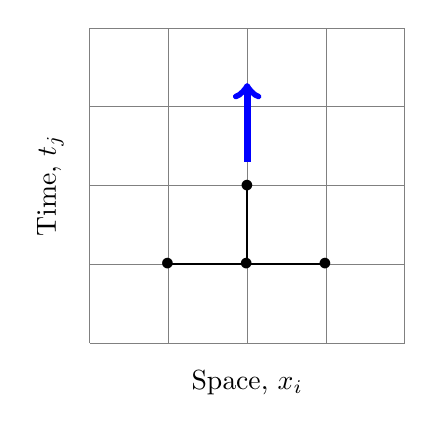
\begin{tikzpicture}
    % Draw the grid
    \draw[very thin, gray] (0,0) grid (4,4);

    % Label the axes
    \node at (2,-0.5) {Space, $x_i$};
    \node[rotate=90] at (-0.5, 2) {Time, $t_j$};

    \foreach \x in {1,2,3} {
        \node at (\x-0.012, 1) {$\bullet$};
    }

    \foreach \x in {1,2} [
        \draw[-, line width=0.05em, black] (\x, 1) -- (\x+1, 1);
    ]

    \draw[-, line width=0.05em, black] (2, 1) -- (2, 2);

    \draw[->, line width=0.25em, blue] (2, 2.3) -- (2, 3.3);
    \node at (2,2-0.012) {$\bullet$}; % Only one point in time step 2 (k=2)
    \end{tikzpicture}
    \caption{Explicit method for the heat equation}
    \label{fig:heat-explicit}
\end{figure}

This is what is known as the explicit scheme.

\subsubsection{Black-Scholes equation}
Similar to the heat equation, the Black Scholes-equation can be discretized to a finite grid of points. For this instance, the domain is defined by time $t \in [0, T]$ (where T represents the expiration time of an option) and asset price $S \in [0,S_{max}]$ (where $S_{max}$ is a sufficiently large upper limit for the underlying asset price). This can be represented by a mesh grid of points.
The time interval $t \in [0, T]$ is divided into $M$ equal-sized time steps, each of size ${\Delta t} = \frac{T}{M}$. Similarly, the asset price range $S \in [0,S_{max}]$ is divided into $N$ equal-sized asset steps, each of size ${\Delta S} = \frac{S_{max}}{N}$.

The price of the option at the current time step will be denoted by $V_i^k$, where $i$ refers to the index representing the asset price grid point  
and $k$ refers to the index representing the time step.

From this, it can be said that the grid points are made up of:
\[
S_i = i {\Delta S},\, t_k = T - k {\Delta t},
\]
where
\[
0 \leq i \leq N \quad \text{and} \quad 0 \leq k \leq M.
\]

Like, in the previous section, the grid can be used to compute an approximation of the option price at the subsequent time step using known values from the current time step. The Black-Scholes equation represents a \textit{backwards} parabolic equation which implies that the subsequent option prices are computed starting from the time at expiration ($t = T$). 

For simplicity, the Black-Scholes equation can be rewritten as such:
\[
\frac{\partial V}{\partial t} + a(S,t) \frac{\partial^2 V}{\partial S^2} + b(S,t) \frac{\partial V}{\partial S} - c(S,t) V = 0
\]
Finite difference approximations will be used to substitute the derivatives of the Black-Scholes PDE:
\begin{align}
\frac{\partial V}{\partial t} &\approx \frac{V_i^k - V_i^{k+1}}{\Delta t} \tag{Theta} \label{eq: theta} \\
\frac{\partial V}{\partial S} &\approx \frac{V_{i+1}^k - V_{i-1}^k}{2 \Delta S} \tag{Delta} \label{eq: delta}\\
\frac{\partial^2 V}{\partial S^2} &\approx \frac{V_{i+1}^k - 2V_i^k + V_{i-1}^k}{\Delta S^2} \tag{Gamma}\label{eq: gamma}
\end{align}
Substituting these three approximations, \eqref{eq: theta}, \eqref{eq: delta}, and \eqref{eq: gamma} into the equation gives us the following:
\[
\frac{V_i^k - V_i^{k+1}}{\Delta t} + a(S,t) \frac{V_{i+1}^k - 2V_i^k + V_{i-1}^k}{(\Delta S)^2} + b(S,t) \frac{V_{i+1}^k - V_{i-1}^k}{2 \Delta S} - c(S,t) V_i^k = 0
\]
The equation is then rearranged such that the $k+1$ terms and $k$ terms are separated:
\[
V_i^{k+1} = A_i^k V_{i-1}^k + (1-B_i^k) V_i^k + C_i^k V_{i+1}^k
\]
{\color{red}What is O?}
where
\begin{align*}
    A_i^k &= a_i^k v_1 - \frac{1}{2} b_i^k v_2 \\
    B_i^k &= -2a_i^k v_1 + c_i^k \Delta t \\
    C_i^k &= a_i^k v_1 + \frac{1}{2} b_i^k v_2 \\
    v_1 &= \frac{\Delta t}{(\Delta S)^2}, \quad v_2 = \frac{\Delta t}{\Delta S}
\end{align*}
The $O(\Delta t^2, \Delta t (\Delta S)^2)$ notation represents the local truncation error.
{\color{red}SO WHAT????!!!! What is the meaning of \textbf{local}?}

The grid below illustrates how the option price at the subsequent time step can be calculated using the neighbouring grid points.


\begin{figure}[H]
    \centering
    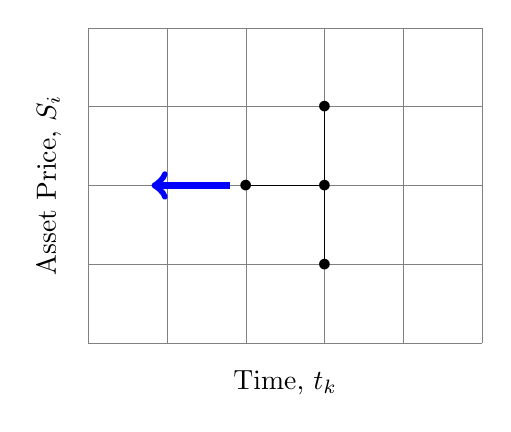
\begin{tikzpicture}
    % Draw the grid
    \draw[very thin, gray] (0,0) grid (5,4);

    % Label the axes
    \node at (2.5,-0.5) {Time, $t_k$};
    \node[rotate=90] at (-0.5, 2) {Asset Price, $S_i$};

    \foreach \y in {1,2,3} {
        \node at (3, \y-0.012) {$\bullet$};
    }
    
    \foreach \y in {1, 2} {
        \draw[-, line width=0.05em, black] (3, \y) -- (3, \y+1);
    }

    \draw[-, line width=0.05em, black] (2, 2) -- (3, 2);

    \draw[->, line width=0.25em, blue] (1.8, 2) -- (0.8, 2);
    \node at (2,2-0.012) {$\bullet$}; 
    \end{tikzpicture}
    \caption{Explicit method for the Black-Scholes equation}
    \label{fig:bse-explicit}
\end{figure}

\subsection{Implicit Scheme: Crank-Nicolson Method}
Despite its straightforward implementation, the explicit method tends to be less stable, as it only takes the current time steps into account for computation. The Crank-Nicolson method addresses this problem by using a combination of the current and subsequent time steps, making it unconditionally stable. It is not confined to the same stability constraints that the explicit method faces.

\subsubsection{Heat equation}
The Crank-Nicolson method involves the approximation of the derivatives at the midpoint of the current and subsequent time steps. By averaging the spatial
second derivatives of both time steps, the following equation is obtained:
\begin{equation}
    \frac{u_i^{j+1} - u_i^j}{\Delta t} = \frac{1}{2(\Delta t)^2} (u_{i+1}^{j+1} - 2u_i^{j+1} + u_{i-1}^{j+1} + u_{i+1}^j - 2u_i^j + u_{i-1}^j),
\end{equation}
which can be rearranged to give
\begin{equation}
    u_i^{j+1} = u_i^j + \frac{\Delta t}{2(\Delta t)^2} (u_{i+1}^{j+1} - 2u_i^{j+1} + u_{i-1}^{j+1} + u_{i+1}^j - 2u_i^j + u_{i-1}^j).
\end{equation}
The equation can be further rewritten to separate the $j+1$ and $j$ terms:
\begin{equation}
    -r u_{i-1}^{j+1} + (1 + 2r) u_i^{j+1} - r u_{i+1}^{j+1} = r u_{i-1}^j + (1 - 2r) u_i^j + r u_{i+1}^j,
\end{equation}
where $r = \frac{\Delta t}{2(\Delta x)^2}$. This leaves us with a tridiagonal system of equations that can be solved to obtain the temperature at the next time step $u_i^{j+1}$.

\begin{figure}[H]
    \centering
    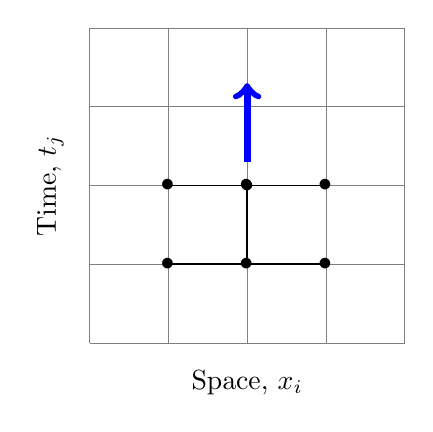
\begin{tikzpicture}
    % Draw the grid
    \draw[very thin, gray] (0,0) grid (4,4);

    % Label the axes
    \node at (2,-0.5) {Space, $x_i$};
    \node[rotate=90] at (-0.5, 2) {Time, $t_j$};

    \foreach \x in {1,2,3} {
        \node at (\x-0.012, 1) {$\bullet$};
        \node at (\x-0.012, 2) {$\bullet$};
    }

    \foreach \y in {1, 2} {
        \draw[-, line width=0.05em, black] (1, \y) -- (3, \y); % Horizontal lines
    }

    \draw[-, line width=0.05em, black] (2, 1) -- (2, 2);

    \draw[->, line width=0.25em, blue] (2, 2.3) -- (2, 3.3);
    \node at (2,2-0.012) {$\bullet$}; % Only one point in time step 2 (k=2)
    \end{tikzpicture}
    \caption{Crank-Nicolson method for the heat equation}
    \label{fig:heat-cn}
\end{figure}


\subsubsection{Black-Scholes equation}
% this needs to be fixed because i use the other way 
Similarly, the Crank-Nicolson method can be applied to the Black-Scholes equation. The equation is rewritten as 
\begin{equation}
    \frac{V_i^{k+1} - V_i^k}{\Delta t} = \frac{1}{2} \left( \mathcal{L}(V_i^{k+1}) + \mathcal{L}(V_i^k) \right)
\end{equation}
such that $\mathcal{L}$ refers to discretized form of the operator that describes how the option value changes. Recall that the following approximations are used for discretization:
\begin{align}
    \frac{\partial V}{\partial t} &\approx \frac{V_i^k - V_i^{k+1}}{\Delta t} \tag{Theta} \\
    \frac{\partial V}{\partial S} &\approx \frac{V_{i+1}^k - V_{i-1}^k}{2 \Delta S} \tag{Delta} \\
    \frac{\partial^2 V}{\partial S^2} &\approx \frac{V_{i+1}^k - 2V_i^k + V_{i-1}^k}{(\Delta S)^2} \tag{Gamma}
 \end{align}
Combine the Explicit (forward) and Implicit (backward) schemes: 
\[
\begin{aligned}
    &\frac{V_i^n - V_i^{n+1}}{\Delta t} + \frac{a_i^{k+1}}{2} \left( \frac{V_{i+1}^{k+1} - 2 V_i^{k+1} + V_{i-1}^{k+1}}{(\Delta S)^2} \right) + \frac{b_i^{k+1}}{2} \left( \frac{V_{i+1}^{k+1} - V_{i-1}^{k+1}}{2 \Delta S} \right) + \frac{1}{2} c_i^{k+1} V_i^{k+1} \\
    &+ \frac{a_i^{k}}{2} \left( \frac{V_{i+1}^{k} - 2 V_i^{k} + V_{i-1}^{k}}{(\Delta S)^2} \right) + \frac{b_i^{k}}{2} \left( \frac{V_{i+1}^{k} - V_{i-1}^{k}}{2 \Delta S} \right) + \frac{1}{2} c_i^{k} V_i^{k} = 0
\end{aligned}
\]
Remove the denominators and rearrange the equation such that the $k+1$ and $k$ terms are separated:
\[
    A_i^{k+1} V_{i-1}^{k+1} + (1+B_i^{k+1})V_i^{k+1} + C_i^{k+1} V_{i+1}^{k+1} = -A_i^k V_{i-1}^{k} + (1-B_i^{k})V_i^{k} + C_i^{k} V_{i+1}^k
\]
where
\begin{align*}
    &A_i^k = \frac{b_i^k v_2}{4} - \frac{a_i^k v_1}{2} \\
    &B_i^k = a_i^k v_1 - \frac{c_i^k}{2} \Delta t \\
    &C_i^k = - \frac{a_i^k v_1}{2} -\frac{b_i^k v_2}{4} \\
    &v_1 = \frac{\Delta t}{(\Delta S)^2}, \quad v_2 = \frac{\Delta t}{\Delta S}
\end{align*}

This is a linear system of equations written in the matrix form of:
\[
    AV^{k+1} = BV^{k}
\]
where $A$ and $B$ represent tridiagonal matrices, and $V^{k+1}$ and $V^{k}$ are vectors containing the option values at the next and current time steps. It is important to note that this is used to solve the interior grid points and only applies to $1 \leq i \leq N_s - 1$, as the boundary conditions address the remaining equations. $N_s$ here refers to the total number of spatial grid points.

This system of equations can be solved to obtain the option values at the next time step $V^{k+1}$.

{\color{red} a few notes about the errors (local/global)?}

\begin{figure}[H]
    \centering
    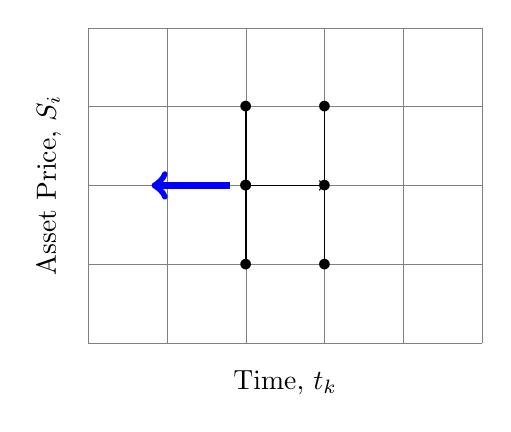
\begin{tikzpicture}
    % Draw the grid
    \draw[very thin, gray] (0,0) grid (5,4);

    % Label the axes
    \node at (2.5,-0.5) {Time, $t_k$};
    \node[rotate=90] at (-0.5, 2) {Asset Price, $S_i$};

    \foreach \y in {1,2,3} {
        \node at (3, \y-0.012) {$\bullet$};
        \node at (2, \y-0.012) {$\bullet$};
    }
    
    \foreach \y in {1, 2} {
        \draw[-, line width=0.05em, black] (2, \y) -- (2, \y+1);
        \draw[-, line width=0.05em, black] (3, \y) -- (3, \y+1);
    }

    \draw[->, line width=0.05em, black] (2, 2) -- (3, 2);
    \draw[->, line width=0.25em, blue] (1.8, 2) -- (0.8, 2);

    \node at (2,2-0.012) {$\bullet$}; 
    \end{tikzpicture}
    \caption{Crank-Nicolson method for the Black-Scholes equation}
    \label{fig:bse-cn}
\end{figure}


\section{Stochastic differential equations}
\subsection{Brownian motion}
\subsection{Ito processes}
\subsection{Geometric Brownian motion}
\subsection{GBM for option pricing}

